\chapter{Metodología}
\lettrine{E}{}l trabajo analítico de este proyecto de investigación se realizó en el Laboratorio de Geoquímica Isotópica y Geocronología (LGIG) del Instituto de Ciencias del Mar y Limnología, Universidad Nacional Autónoma de México - Unidad Académica Mazatlán, Sinaloa, México. El LGIG cuenta con sistemas de espectrometría de rayos gamma (Sección \ref{Secc-EspectrometriaGamma}), XRF (Sección \ref{Secc-EspectrometriaXRF}) y analizador elemental de carbono - nitrógeno, C-N (Sección \ref{Secc-CN})  que permiten obtener información sobre la composición elemental y la actividad de diversos radionúclidos (Tabla \ref{Table-MaterialesRef}). 
\\
\\
Los análisis elementales mediante XRF y C-N permiten proponer un método para estimar el 100 \% de la composición elemental de los sedimentos (Sección \ref{Secc-100Composicion}). Esta información, junto con la densidad de la muestra, permite corregir la actividad medida de las muestras utilizando el software ANGLE, Sección \ref{SubSec-ANGLE}.
\\
\\
El proyecto se centró en seis núcleos sedimentarios, pertenecientes a ecosistemas acuáticos de México: un lago cráter, el Golfo de México, el mar Caribe y el océano Pacífico (Sección \ref{Secc-ZonasSeleccionadas}). En la Sección \ref{Secc-Codigos} se describen los códigos de programación desarrollados para la lectura de  los datos experimentales y el cálculo sistemático de la eficiencia mediante ANGLE.
	\section{Sistemas de espectrometría de rayos gamma}\label{Secc-EspectrometriaGamma}
El LGIG posee cuatro sistemas de espectrometría de rayos gamma idenfiticados como G1, G2, G3 y G4. Cada sistema está compuesto por un detector de Ge hiper-puro en configuración tipo pozo (Sección \ref{SubSecc-DetecGe}), un blindaje pasivo (Sección \ref{SubSec-Blindaje}), un sistema de refrigeración (sección \ref{SubSec-Refrigeracion}) y electrónica asociada (Sección \ref{SubSec-Electronica}).
\\ 
\\ 
Cada sistema de espectrometría de rayos gamma se caracteriza por el espectro de fondo (Sección \ref{SubSec-Fondos}) y las calibraciones: canal - energía, eficiencia - energía. Para realizar y comprobar estas calibraciones se utilizaron una solución patrón de emisores gamma, un material de referencia Uranio - Torio ORE DL1a y Materiales de Referencia Certificados (Sección \ref{SubSec-MaterialesDeReferencia}). Las calibraciones se presentan en la Sección \ref{SubSec-CaliChannel}. 
\\
\\
El análisis de los espectros energéticos de rayos gamma se realizó mediante el software \textit{GammaVision}, versión 7.02.01, marca ORTEC. La sección \ref{SubSec-GammaVision} muestra las características y los ajustes utilizados en GammaVision. 
		\subsection[Detectores de Ge hiper-puro]{Detector de Ge hiper-puro en configuración tipo pozo}\label{SubSecc-DetecGe}
Los detectores de germanio hiper-puro son de tipo pozo y marca ORTEC. Las características principales, los parámetros geométricos necesarios para determinar la eficiencia mediante ANGLE y el modelo de cada detector se presentan en la Figura \ref{Fig-DetectorGeEsquema} y en la Tabla \ref{Tabla-Dimensiones-Detectores}. Todos los detectores tienen una profundidad de 40 mm y un diámetro de pozo efectivo de 15.5 mm.
\begin{figure}[h]
\centering
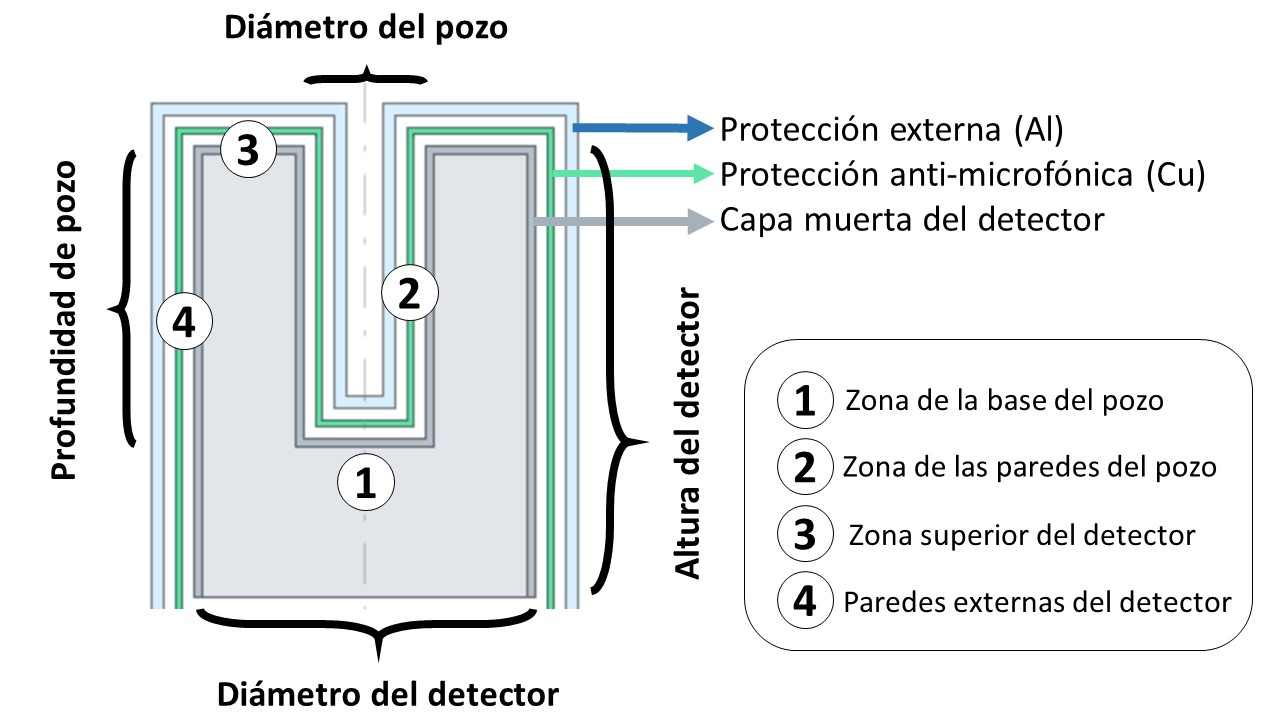
\includegraphics[width=\textwidth]{Imagenes/Zona_Detector_Ge.jpg}
\caption{Variables y zonas necesarias para especificar las dimensiones de los detectores de Ge hiper-puro en configuración pozo del LGIG.}\label{Fig-DetectorGeEsquema}
\end{figure}
\begin{table}
\caption{Características principales de los detectores de germanio hiper-puro en configuración tipo pozo. Las variables y zonas se detallan en la Figura \ref{Fig-DetectorGeEsquema}.}\label{Tabla-Dimensiones-Detectores}
\centering
\begin{tabular}{|c|c|c|c|c|c|}\hline
\rowcolor{Blue3}		&	Unidades	&	G1	&	G2	&	G3	&	G4	\\	\hline	\hline
\rowcolor{Blue2}	\multicolumn{2}{|c}{Dimensiones del cristal de Ge }			&		&		&		&		\\	\hline	
\rowcolor{Blue1}	Altura del detector	&	mm	&	64.8	&	66.5	&	69.7	&	69.1	\\		
\rowcolor{Blue1}	Diámetro del detector	&	mm	&	54.6	&	54.6	&	66.7	&	61.6	\\		
\rowcolor{Blue1}	Profundidad de pozo 	&	mm	&	55.6	&	53.5	&	56.7	&	55.1	\\		
\rowcolor{Blue1}	Diámetro de pozo 	&	mm	&	11.4	&	10.55	&	10.5	&	10.95	\\		
\rowcolor{Blue1}	Volumen activo	&	cc	&	124	&	124	&	206	&	169	\\	\hline	\hline
\rowcolor{Blue2}	\multicolumn{2}{|c}{Capa muerta de Ge }			&		&		&		&		\\	\hline	
\rowcolor{Blue1}	Zona 1	&	mm	&	$3\times 10^{-5}$	&	$3\times 10^{-5}$	&	$3\times 10^{-5}$	&	$3\times 10^{-5}$	\\		
\rowcolor{Blue1}	Zona 2	&	mm	&	$3\times 10^{-5}$	&	$3\times 10^{-5}$	&	$3\times 10^{-5}$	&	$3\times 10^{-5}$	\\		
\rowcolor{Blue1}	Zona 3	&	mm	&	0	&	$3\times 10^{-5}$	&	0	&	0	\\		
\rowcolor{Blue1}	Zona 4	&	mm	&	0.7	&	0.7	&	0	&	0.7	\\	\hline	\hline
\rowcolor{Blue2}	\multicolumn{2}{|c}{Protección anti-microfónica (Cu)}			&		&		&		&		\\	\hline	
\rowcolor{Blue1}	Zona 3	&	mm	&	1.6	&	1.6	&	1.6	&	1.6	\\	\hline	\hline
\rowcolor{Blue2}	\multicolumn{2}{|c}{Protección externa (Al)}			&		&		&		&		\\	\hline	
\rowcolor{Blue1}	Zona 1	&	mm	&	1	&	1	&	1	&	2.032	\\		
\rowcolor{Blue1}	Zona 2	&	mm	&	0.5	&	0.5	&	0.5	&	0.5	\\		
\rowcolor{Blue1}	Zona 3	&	mm	&	2.032	&	2.032	&		&	2.032	\\	\hline	\hline
\rowcolor{Blue2}	\multicolumn{2}{|c}{Distancia entre Al y Cu}			&		&		&		&		\\	\hline	
\rowcolor{Blue1}	Zona 1	&	mm	&	7.8	&	3.125	&	7.92	&	3.9	\\		
\rowcolor{Blue1}	Zona 2	&	mm	&	1.8	&	1.15	&	1.3	&	1.3	\\		
\rowcolor{Blue1}	Zona 3	&	mm	&	6.4	&	8.4	&	4.2	&	8.39	\\	\hline	\hline
\rowcolor{Blue2}	\multicolumn{2}{|c}{Distancia entre Cu y Ge}			&		&		&		&		\\	\hline	
\rowcolor{Blue1}	Zona 1	&	mm	&	7.8	&	3.125	&	7.92	&	3.99	\\		
\rowcolor{Blue1}	Zona 2	&	mm	&	1.8	&	1.15	&	1.3	&	1.3	\\		
\rowcolor{Blue1}	Zona 3	&	mm	&	0.2	&	0.279	&	4.2	&	0.279	\\	\hline	\hline
\rowcolor{Blue2}	Voltaje operativo	&	V	&	+2500	&	+2500	&	+1500	&	+3600	\\	\hline	\hline
\rowcolor{Blue1} Modelo & GWL- & 120-15-5 & 120-15-LB-AWT & \multicolumn{2}{c|}{150-15-LB-AWT}\\ \hline
\end{tabular}
\begin{flushleft}
Zona 1: parte inferior del pozo. \\
Zona 2: lateral del pozo.  \\
Zona 3: parte superior del detector. \\
Zona 4: parte lateral externa del detector.
\end{flushleft}
\end{table}
		\subsection{Blindaje de la radiación}\label{SubSec-Blindaje}
Los detectores de Ge hiper-puro del LGIG cuentan con blindaje pasivo (HPLBS - High Performance Low Background Lead Shields, ORTEC). El blindaje es cilíndrico, con $\sim$ 10 cm  de plomo de bajo fondo, y dos capas de Cu y Sn para la absorción de los rayos X generados en el blindaje de plomo \cite{OrtecShield}. La parte inferior del blindaje contiene una apertura circular por donde se comunica el detector con el sistema de refrigeración y la electrónica asociada.		
		\subsection{Sistema de refrigeración}\label{SubSec-Refrigeracion}
Cada sistema de espectrometría de rayos gamma se refrigera con un sistema de condensación de nitrógeno líquido (MÖBIUS Recycler, ORTEC), constituido por un dewar, un sistema de presión de vapor y un condensador criogénico que reutiliza el nitrógeno manteniendo la presión de vapor constante a 3.5 kPa \cite{Mobius}. La capacidad de almacenamiento de nitrógeno líquido es de 28 L y requiere ser rellenado aproximadamente una vez al año, dadas las condiciones ambientales de Mazatlán, Sinaloa, México.
		\subsection{Electrónica asociada}\label{SubSec-Electronica}
Cada detector cuenta en su base con un preamplificador que recibe la carga creada por la interacción de los rayos gamma de la muestra y el cristal de Ge. La señal es transmitida a la electrónica integrada \textit{DSPEC jr 2.0} (ORTEC), que integra una fuente de tensión de alto voltaje, un amplificador, un analizador multicanal y un convertidor análogo - digital (ADC).
\\
\\
En la  Figura \ref{Fig-G1System} se aprecian el sistema de refrigeración, el blindaje, el recubrimiento externo del cristal de Ge hiper-puro (Cu y Al) y el recubrimiento interior del sistema de blindaje (Cu).
\begin{figure}[h]
\centering
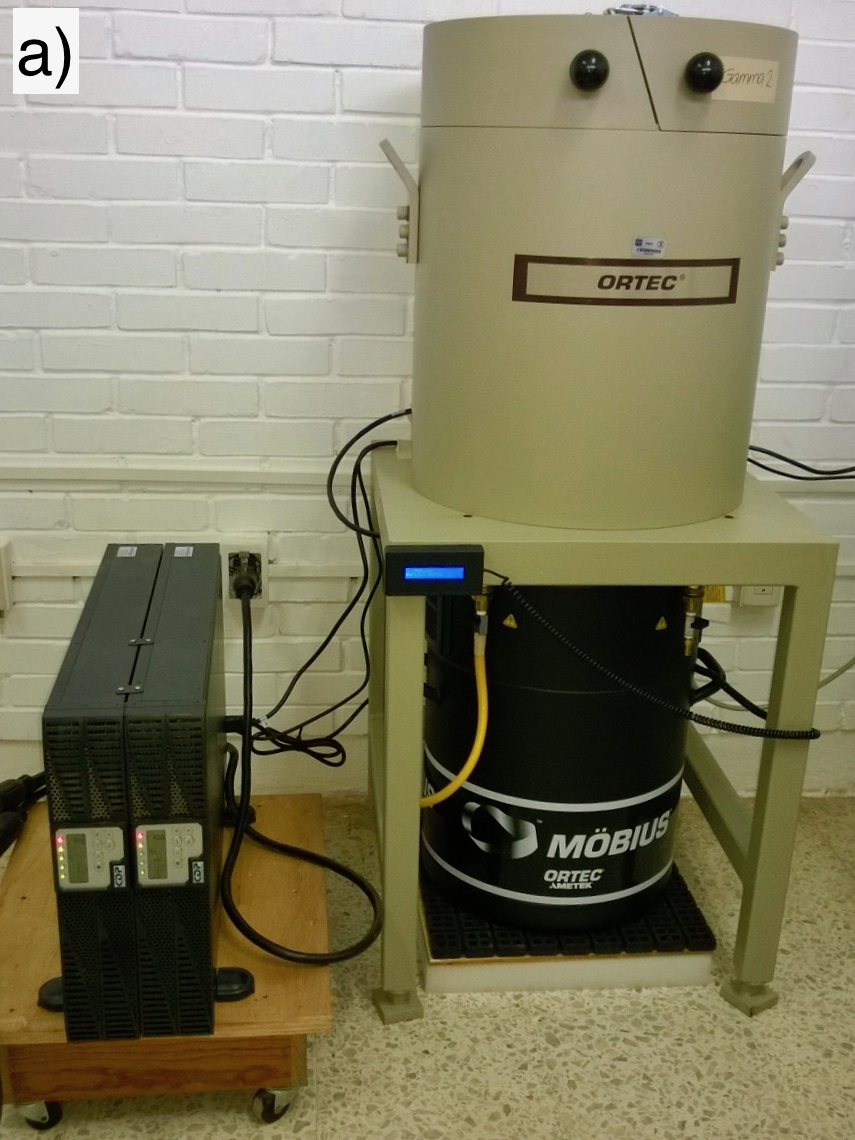
\includegraphics[height=0.4\textheight]{Imagenes/GammaSystem.jpg}
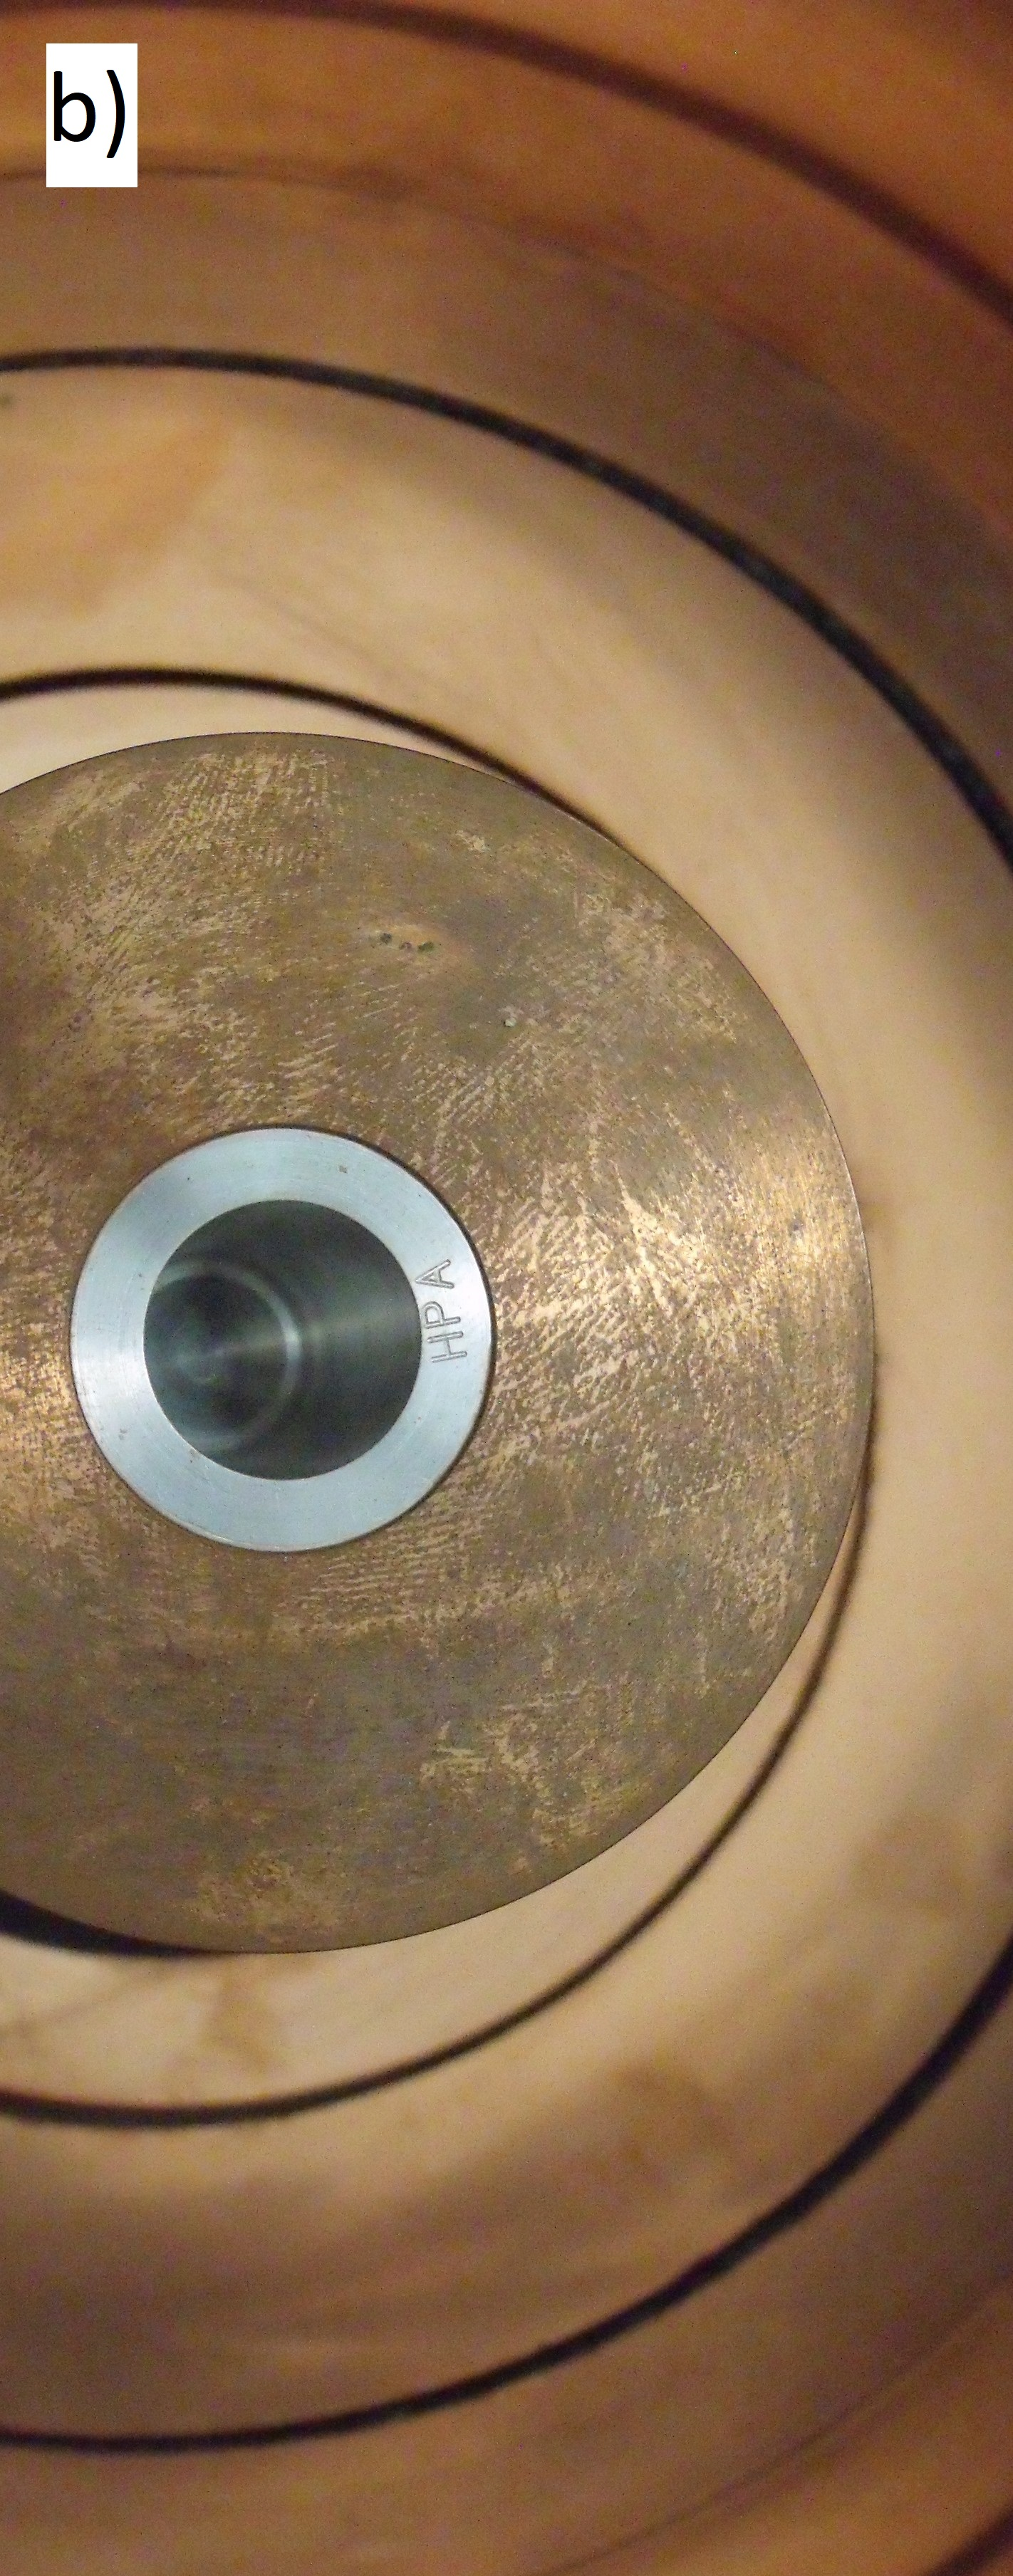
\includegraphics[height=0.4\textheight]{Imagenes/DSCF1886.jpg}
\caption{Sistema de espectrometría de rayos gamma G2 del LGIG. a) Sistema de refrigeración, blindaje y fuente de alimentación. b) Detector de Ge hiper-puro dentro de blindaje.}\label{Fig-G1System}
\end{figure}
		\subsection{Espectro del fondo}\label{SubSec-Fondos}
El espectro de fondo de cada sistema de espectrometría de rayos gamma del LGIG es medido durante aproximadamente dos semanas. En general, se pueden observar radionúclidos antropogénicos ($^{60}$Co y $^{137}$Cs), primordiales ($^{235}$U, $^{238}$U, $^{232}$Th, $^{40}$K) y de rayos cósmicos, entre otros \cite{gilmore2008}. Cada espectro medido debe ser corregido con el espectro de fondo correspondiente. 
\\
\\
En los espectros de fondos de los sistemas de espectrometría gamma del LGIG (Figura \ref{Fig-Fondos}) se observa claramente los radionúclidos primordiales \Kcuarenta, \PbCuatro\, y \BiCuatro, descendientes de \UDosTresOcho\, (Figura \ref{Fig-SerieUranio}). El mayor fondo del detector G1 es debido a que no se trata de un detector con configuración de bajo fondo, y el mayor fondo de los detectores G3 y G4 es debido a su mayor volumen activo. 
\\
\\
La Tabla \ref{Table-CuentasBackground} muestra el número de cuentas del fondo para cada uno de los sistemas de espectrometría de rayos gamma en las energías de interés. El tiempo muerto de la detección de rayos gammas es, en la mayoría de los casos, inferior al 1 \% debido a la baja actividad de las muestras ambientales analizadas en el presente trabajo. Por lo anterior, también se espera que el efecto de \textit{pile-up} sea despreciable y en todo caso, corregido por el sistema electrónico \textit{DSPEC jr 2.0} (ORTEC). 
\begin{figure}[h]
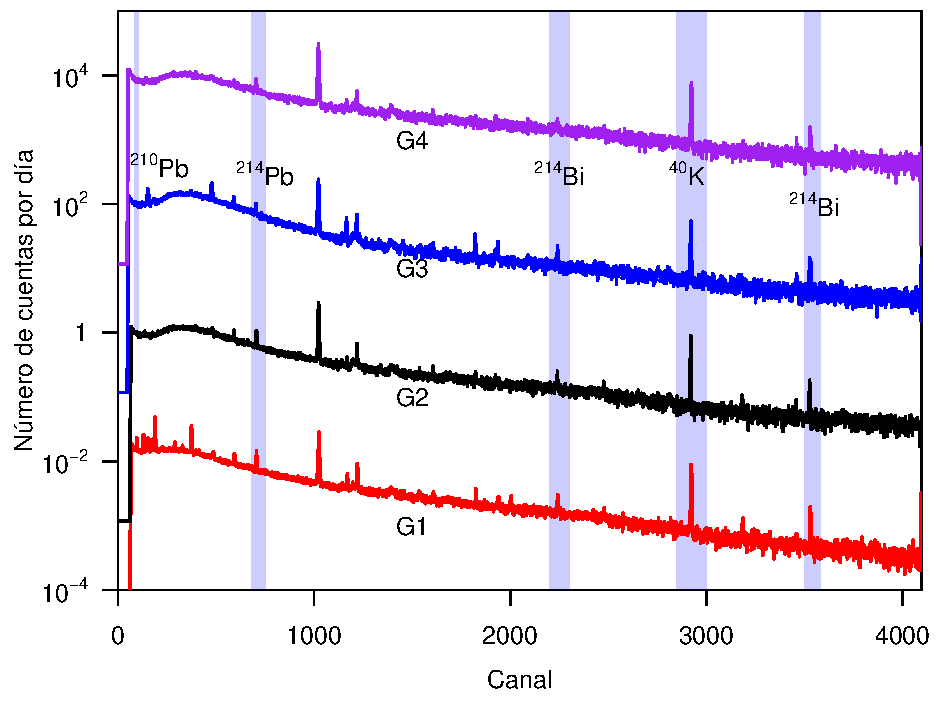
\includegraphics[width=0.9\textwidth]{Imagenes/Fondos.pdf}
\caption{Espectro del fondo para los sistemas de espectrometría de rayos gamma del LGIG.}\label{Fig-Fondos}
\end{figure}
\begin{table}[h]
\centering
\caption{Tasa de cuentas del espectro de fondo para las energías de interés y para cada uno de los sistemas de espectrometría de rayos gamma del LGIG.}\label{Table-CuentasBackground}
\begin{tabular}{|c|c|c|c|c|c|}
	\hline												
\rowcolor{Blue2}	Energía 	&	Radionúclido 	&	G1	&	G2	&	G3	&	G4	\\	\hline
	keV	&		&	 \multicolumn{4}{c|}{Número de cuentas por segundo}           							\\	\hline
\rowcolor{Blue1}	46.54	&	$^{210}$Pb	&	0.003	&	0	&	0	&	0	\\	
\rowcolor{Blue1}	351.99	&	$^{214}$Pb	&	0.003	&	0.001	&	0.004	&	0.001	\\	\hline
\end{tabular}
\end{table}
		\subsection{Materiales de Referencia Certificados}\label{SubSec-MaterialesDeReferencia}
El LGIG cuenta con materiales de referencia utilizados para realizar y comprobar las calibraciones de energía y eficiencia. Se utiliza una solución acuosa patrón de emisores gamma y un material de referencia Uranio - Torio ORE DL1a para realizar las calibraciones en eficiencia y energía. En la Tabla \ref{Table-MaterialesRef} se muestran las características de esta solución y de otros radionúclidos de interés para el LGIG. Por otra parte, la validación de las calibraciones se realiza con Materiales de Referencia Certificados que se muestran en la Tabla \ref{Table-OtrosMaterialesRefIAEA}.
\begin{table}[h]
\centering
\caption{Características de los radionúclidos del material de referencia Mix-Gamma y otros radionúclidos de interés para el LGIG (con $^{*}$): núcleo progenitor y núcleo descendiente, proceso nuclear de desintegración o des-excitación y energía del rayo gamma emitido.}\label{Table-MaterialesRef}
\begin{tabular}{|c|c|c|c|c|c|c|}
\hline																
\rowcolor{Blue3}		\begin{tabular}{@{}c@{}}Núcleo \\ progenitor \end{tabular}	&	$T_{\frac{1}{2}}$       	&	\begin{tabular}{@{}c@{}}Proceso \\ nuclear \end{tabular}	&	\begin{tabular}{@{}c@{}}Núcleo \\ descendiente \end{tabular}	&	 \multicolumn{2}{|c|}{\begin{tabular}{@{}c@{}} Energía del estado \\ inicial y final  \end{tabular} }           			&	\begin{tabular}{@{}c@{}}Energía\\ de rayo \\ gamma \end{tabular}	\\ 	\hline
			&		&		&		&	keV	&	keV	&	keV	\\ 	\hline
\rowcolor{Blue2}		 \multicolumn{7}{|c|}{Mix-Gamma}           													\\ 	\hline
\rowcolor{Blue1}	\cellcolor{Green3}	$^{241}$Am$^{*}$	&	432.6 años	&	$\alpha$	&	 	$^{237}$Np	 	&	 	59.54	 	&	 	0	 	&	\cellcolor{Green3} 59.54	\\ 	
\rowcolor{Blue1}		 	$^{109}$Cd	 	&	 	461.9 días 	 	&	C. E.	&	 	$^{109}$Ag	 	&	 	88.04	 	&	 	0	 	&	88.04	\\ 	
\rowcolor{Blue1}		 	$^{57}$Co	 	&	 	271.8 días	 	&	C. E.	&	 	$^{57}$Fe	 	&	 	136.47	 	&	 	14.41	 	&	122.06	\\ 	
\rowcolor{Blue1}		 	$^{139}$Ce	 	&	 	137.6 días	 	&	C. E.	&	 	$^{139}$La	 	&	 	165.86	 	&	 	0	 	&	165.86	\\ 	
\rowcolor{Blue1}		 	$^{203}$Hg	 	&	 	46.59 días	 	&	$\beta^-$	&	 	$^{203}$Tl	 	&	 	279.19	 	&	 	0	 	&	279.19	\\ 	
\rowcolor{Blue1}		 	$^{113}$Sn	 	&	 	115.1 días	 	&	C. E.	&	 	$^{113}$In	 	&	 	391.69	 	&	 	0	 	&	391.69	\\ 	
\rowcolor{Blue1}		 	$^{134}$Ba	 	&	 		 	&	$\gamma$	&	 	$^{134}$Ba	 	&	 	604.7	 	&	 	0	 	&	604.7	\\ 	
\rowcolor{Blue1}	\cellcolor{Green3}	 	$^{137}$Cs$^{*}$	 	&	 	30.05 años	 	&	$\beta^-$	&	 	$^{137}$Ba	 	&	 	667.66	 	&	 	0	 	&	\cellcolor{Green3} 661.66	\\ 	
\rowcolor{Blue1}	\cellcolor{Green3}	 	$^{134}$Cs	$^{*}$ 	&	 	2.064 años	 	&	$\beta^-$	&	 	$^{134}$Ba	 	&	 	1400.59	 	&	 	604.7	 	&	\cellcolor{Green3} 795.9	\\ 	
\rowcolor{Blue1}		 	$^{54}$Mn	 	&	 	312.2 días	 	&	C. E.	&	 	$^{54}$Cr	 	&	 	834.8	 	&	 	0	 	&	834.8	\\ 	
\rowcolor{Blue1}		 	$^{88}$Y	 	&	 	106.6 días	 	&	C. E.	&	 	$^{88}$Sr	 	&	 	2734.1	 	&	 	1836.1	 	&	989	\\ 	
\rowcolor{Blue1}		 	$^{65}$Zn	 	&	 	244 días	 	&	C. E.	&	 	$^{65}$Cu	 	&	 	1115.5	 	&	 	0	 	&	1115.5	\\ 	
\rowcolor{Blue1}		 	$^{88}$Sr	 	&	 		 	&	$\gamma$	&	 	$^{88}$Sr	 	&	 	1836.1	 	&	 	0	 	&	1836	\\ 	\hline
\rowcolor{Blue2}		 \multicolumn{7}{|c|}{Radionúclidos de interés para el LGIG}           													\\ 	\hline
\rowcolor{Blue1}	\cellcolor{Green3}	$^{7}$Be	&	53.22 días 	&	C. E.	&	$^{7}$Li	&	477.6	&	0	&	\cellcolor{Green3} 477.6	\\ 	
\rowcolor{Blue1}	\cellcolor{Green3}	$^{208}$Tl	&	1.402 $\cdot 10^{10}$ años	&	$\beta^-$	&	$^{208}$Pb	&	3197.71	&	2614.55	&	\cellcolor{Green3} 583.16	\\ 	
\rowcolor{Blue1}	\cellcolor{Green3}	$^{228}$Ac	&	1.402 $\cdot 10^{10}$ años	&	$\beta^-$	&	$^{228}$Th	&	396.08	&	57.76	&	\cellcolor{Green3} 338.32	\\ 	
\rowcolor{Blue1}	\cellcolor{Green3}	$^{40}$K	&	1.25 $\cdot 10^{9}$ años	&	E. C. 	&	$^{40}$Ar	&	1460.851	&	0	&	\cellcolor{Green3} 1460.851	\\ 	
\rowcolor{Blue1}	\cellcolor{Green3}	$^{210}$Pb	&	22.23 años	&	$\beta^-$	&	$^{210}$Bi	&	46.54	&	0	&	\cellcolor{Green3} 46.54	\\ 	
\rowcolor{Blue1}	\cellcolor{Green3}	$^{214}$Pb	&	1600 años	&	$\beta^-$	&	$^{214}$Bi	&	351.93	&	0	&	\cellcolor{Green3} 351.93	\\ 	
\rowcolor{Blue1}	\cellcolor{Green3}	$^{234}$Th	&	4.468 $\cdot 10^{9}$ años	&	$\beta^-$	&	$^{234}$Pa	&	166.72	&	103.42	&	\cellcolor{Green3} 63.3	\\ 	\hline
\end{tabular}
\end{table}
\begin{table}[h]
\centering
\caption{Materiales de Referencia Certificados, MRC.}\label{Table-OtrosMaterialesRefIAEA}
\begin{tabular}{|c|c|}
	\hline								
\rowcolor{Blue2}	MRC	&	Radionúclidos	\\	\hline	
\rowcolor{Blue1}	IAEA 300	&		$^{40}$K, $^{60}$Co, $^{125}$Sb, $^{134}$Cs, $^{155}$Eu, $^{210}$Pb, $^{210}$Po, $^{228}$Ra, $^{234}$U, $^{239,240}$Pu, 	 $^{241}$Am. 	\\	\hline	
\rowcolor{Blue1}	IAEA 313	&	$^{226}$Ra, Th, U.				\\	\hline	
\rowcolor{Blue1}	IAEA 314	&	$^{226}$Ra, Th, U.				\\	\hline	
\rowcolor{Blue1}	IAEA 375	&		$^{40}$K, $^{90}$Sr, $^{106}$Ru, $^{125}$Sb, $^{129}$I, $^{134}$Cs, $^{137}$Cs, $^{226}$Ra, $^{232}$Th. 	\\	\hline	
\rowcolor{Blue1}	IAEA-384	&		\begin{tabular}{@{}c@{}}$^{40}$K, $^{60}$Co, $^{155}$Eu, $^{230}$Th, $^{238}$U,  	$^{238}$Pu, $^{239,2340}$Pu, $^{241}$Am, $^{90}$Sr, $^{137}$Cs,\\  	 $^{210}$Pb, $^{226, 228}$Ra, $^{232}$Th, $^{234, 235}$U, $^{239,240,241}$Pu. \end{tabular}	\\	\hline	
\rowcolor{Blue1}	IAEA-414	&		$^{40}$K, $^{137}$Cs, $^{232}$Th, $^{234,235,238}$U, $^{238, 239+240}$Pu,         	 $^{241}$Am, $^{90}$Sr, $^{210}$Pb, $^{226}$Ra, $^{239,240,241}$Pu.          	\\	\hline	
\rowcolor{Blue1}	IAEA-444	&		$^{54}$Mn, $^{60}$Co, $^{65}$Zn, $^{109}$Cd,      $^{134,137}$Cs, $^{210}$Pb, $^{241}$Am.  \\	\hline	
\rowcolor{Blue1}	IAEA-448	&		 $^{226}$Ra, $^{40}$K, $^{208}$Tl, $^{210, 212}$Pb,     $^{228}$Ac,  $^{232}$Th, $^{235, 238}$U.      \\	\hline	
\rowcolor{Blue1}	DL1a	&	U, Th, $^{226}$Ra, $^{210}$Pb.				\\	\hline	
\rowcolor{Blue1}	KCl	&	$^{40}$K.				\\	\hline	
\end{tabular}
\end{table}
		\subsection{Calibraciones}\label{SubSec-CaliChannel}
Las calibraciones se realizaron para cada detector y dos geometrías. El LGIG usa geometrías según la cantidad disponible de muestra, que se denotan 2 mL y 4 mL. En la Figura \ref{Fig-Cal-Canal-Energia} se observa que las calibraciones canal - energía presentaron una excelente linealidad. 
\\
\\
La Tabla \ref{Tabla-EficienciasPb} muestra los valores de la eficiencia de referencia para las dos energías de interés (46.54 keV y 351.93 keV), los diferentes sistemas de espectrometría (G1, G2, G3 y G4) y dos de las geometrías (2 mL y 4 mL) utilizadas en el LGIG. Una geometría de 2 mL denota un volumen de muestra de 1.939 $\pm$ 0.007 cm$^{3}$ y una geometría de 4 mL denota un volumen de muestra de 4.071 $\pm$ 0.004 cm$^{3}$. La Figura \ref{Fig-EficienciaAgua} muestra algunas curvas de eficiencia referencia (ver Objetivos específicos, Sección \ref{Sec-ObjEspec}) en cada detector y diferentes geometrías.
\\
\\
Para reducir la incertidumbre de la medida debida a la calibración y disponer de actividades lo más exactas posibles, las eficiencias fueron determinadas tan sólo para los radionúclidos de interés (Tabla \ref{Table-MaterialesRef}), por lo que no se propuso una curva de eficiencia continua ni se realizó correcciones debido a la coincidencia de dos rayos gamma asociados al mismo evento de decaimiento, (TCSC, por sus siglas en inglés). En caso de requerir la cuantificación de nuevos radionúclidos, sus eficiencias son determinadas por simulación mediante el software ANGLE (Sección \ref{SubSec-ANGLE}) utilizando puntos de calibración pertenecientes a emisores monoenergéticos y, por lo tanto, no afectadas por correcciones de coincidencia. 
\begin{table}[h]
\centering
\caption{Eficiencia de referencia para \PbCero\,(46.54 keV) y \PbCuatro\,(351.93 keV) de los diferentes sistemas gamma del LGIG para diferentes geometrías (2 mL y 4 mL).}\label{Tabla-EficienciasPb}
\begin{tabular}{|c|c|c|} \hline
\rowcolor{Blue2}	Detector y geometría & $\epsilon$(\PbCero) & $\epsilon$(\PbCuatro) \\ \hline
\rowcolor{Blue1}	G1 - 2 mL & 0.71 & 0.25 \\
\rowcolor{Blue1}	G1 - 4 mL & 0.63 & 0.22 \\
\rowcolor{Blue1}	G2 - 2 mL & 0.71 & 0.25 \\
\rowcolor{Blue1}	G2 - 4 mL & 0.68 & 0.24 \\
\rowcolor{Blue1}	G3 - 2 mL & 0.71 & 0.34 \\
\rowcolor{Blue1}	G3 - 4 mL & 0.64 & 0.30 \\
\rowcolor{Blue1}	G4 - 2 mL & 0.66 & 0.30 \\
\rowcolor{Blue1}	G4 - 4 mL & 0.63 & 0.28 \\ \hline
\end{tabular}
\end{table}
\begin{figure}[h]
\centering
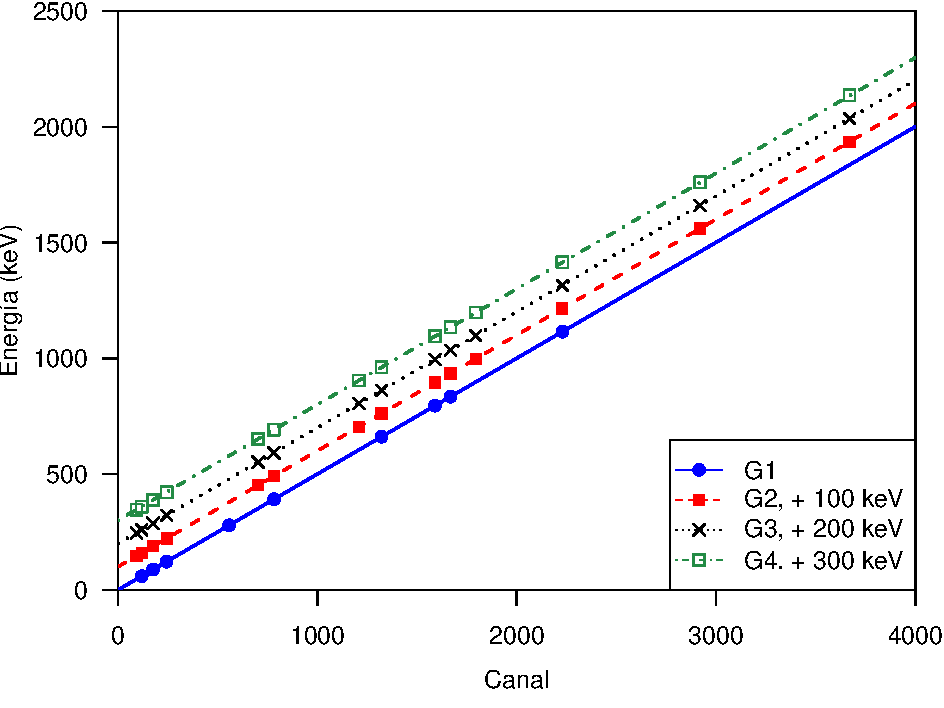
\includegraphics[width=0.7\textwidth]{Imagenes/Calibraciones_Canal_Energia.pdf}
\caption{Calibración canal-energía para los sistemas de espectrometría de rayos gamma del LGIG. Las calibraciones se encuentran desplazadas en + 100 keV, + 200 keV y +300 keV para G2, G3 y G4, respectivamente.}\label{Fig-Cal-Canal-Energia}
\end{figure}
\begin{figure}[h]
\centering
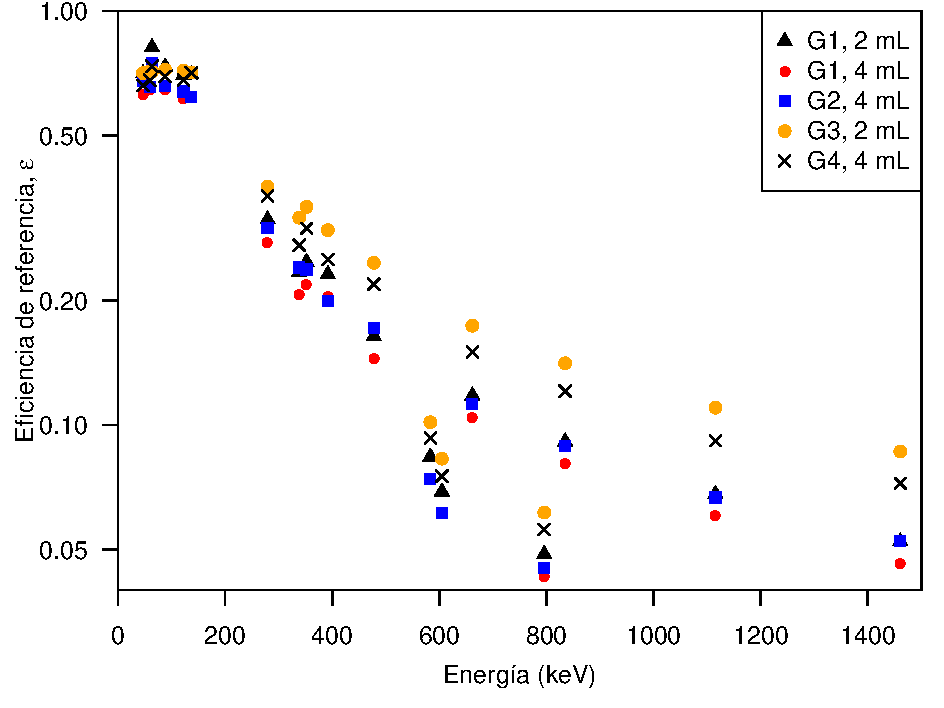
\includegraphics[width=0.7\textwidth]{Imagenes/Eficiencia_agua.pdf}
\caption{Eficiencia de referencia para diferentes detectores y geometrías (2 mL y 4 mL) del LGIG.}\label{Fig-EficienciaAgua}
\end{figure}
		\subsection{GammaVision}\label{SubSec-GammaVision}
El control de la electrónica y el análisis de los espectros energéticos de rayos gamma se realizó mediante el software GammaVision (ORTEC). La búsqueda y el análisis de los fotopicos de interés, y el cálculo de la actividad específica (Bq kg$^{-1}$), se efectuó con base en:
\begin{itemize}
\item Las calibraciones en energía y en eficiencia. 
\item El espectro del fondo.
\item La librería con información nuclear de los radioisótopos de interés. 
\end{itemize}
Algunos parámetros utilizados en el análisis son: \cite{GammaVisionManual}
\begin{itemize}
\item Background type: 3-Point. El cálculo del fondo para un pico se realiza como el promedio del fondo de lado izquierdo (bajas energías) y derecho (altas energías) del centroide de un fotopico. El fondo izquierdo/derecho es definido como el valor mínimo del promedio de tres canales en el intervalo que comprende el canal del centroide $\pm 4\times$ FWHM.
\item MDA Type: Traditional ORTEC. La actividad mínima detectable (MDA) es la estimación de la actividad que, \textit{a priori}, puede proporcionar cada sistema de detección. Su valor depende de la eficiencia, fondo y tiempo de medida. 
\item Peak search sensitivity: 3. La sensibilidad en la búsqueda de picos (entre 1 y 5) permite seleccionar la importancia de los picos que se consideran en el análisis. Un valor bajo (1) puede encontrar muchos picos “falsos” y el valor más alto (5) puede ignorar picos relevantes. 
\item Analysis method: ROI32. El método ROI32 busca picos tan sólo en las zonas de interés (ROI) basándose en la calibración canal – energía. 
\end{itemize} 
\newpage
\newpage
	\section{Espectrometría de fluorescencia de rayos X}\label{Secc-EspectrometriaXRF}
En el LGIG se mide la concentración elemental para $Z>10$ a través de la técnica XRF (Sección \ref{SubSec-XRF-Intro}) mediante el equipo \textit{SPECTRO XEPOS III}. El equipo de medición se muestra en la Figura \ref{Fig-XEPOS}. La cantidad de masa requerida es de 2 a 4 g. La incertidumbre asociada a la medida de la concentración $x_i$ de elemento $i$, $\bigtriangleup x_i$, se calcula utilizando una carta de calidad mediante la relación entre la desviación estándar $\sigma_\text{Referencia}$ y el valor promedio $\overline{x}_\text{Referencia}$ para diferentes mediciones de Materiales de Referencia Certificados. Si $x_i$ es el valor medido de un elemento $i$, entonces la incertidumbre asociada, $\bigtriangleup x_i$, es
\begin{equation}\label{Eq-SigmaRef}
\bigtriangleup x_i = \dfrac{\sigma_\text{Referencia}}{\overline{x}_\text{Referencia}}\times x_i.
\end{equation}
\begin{figure}[h]
\centering
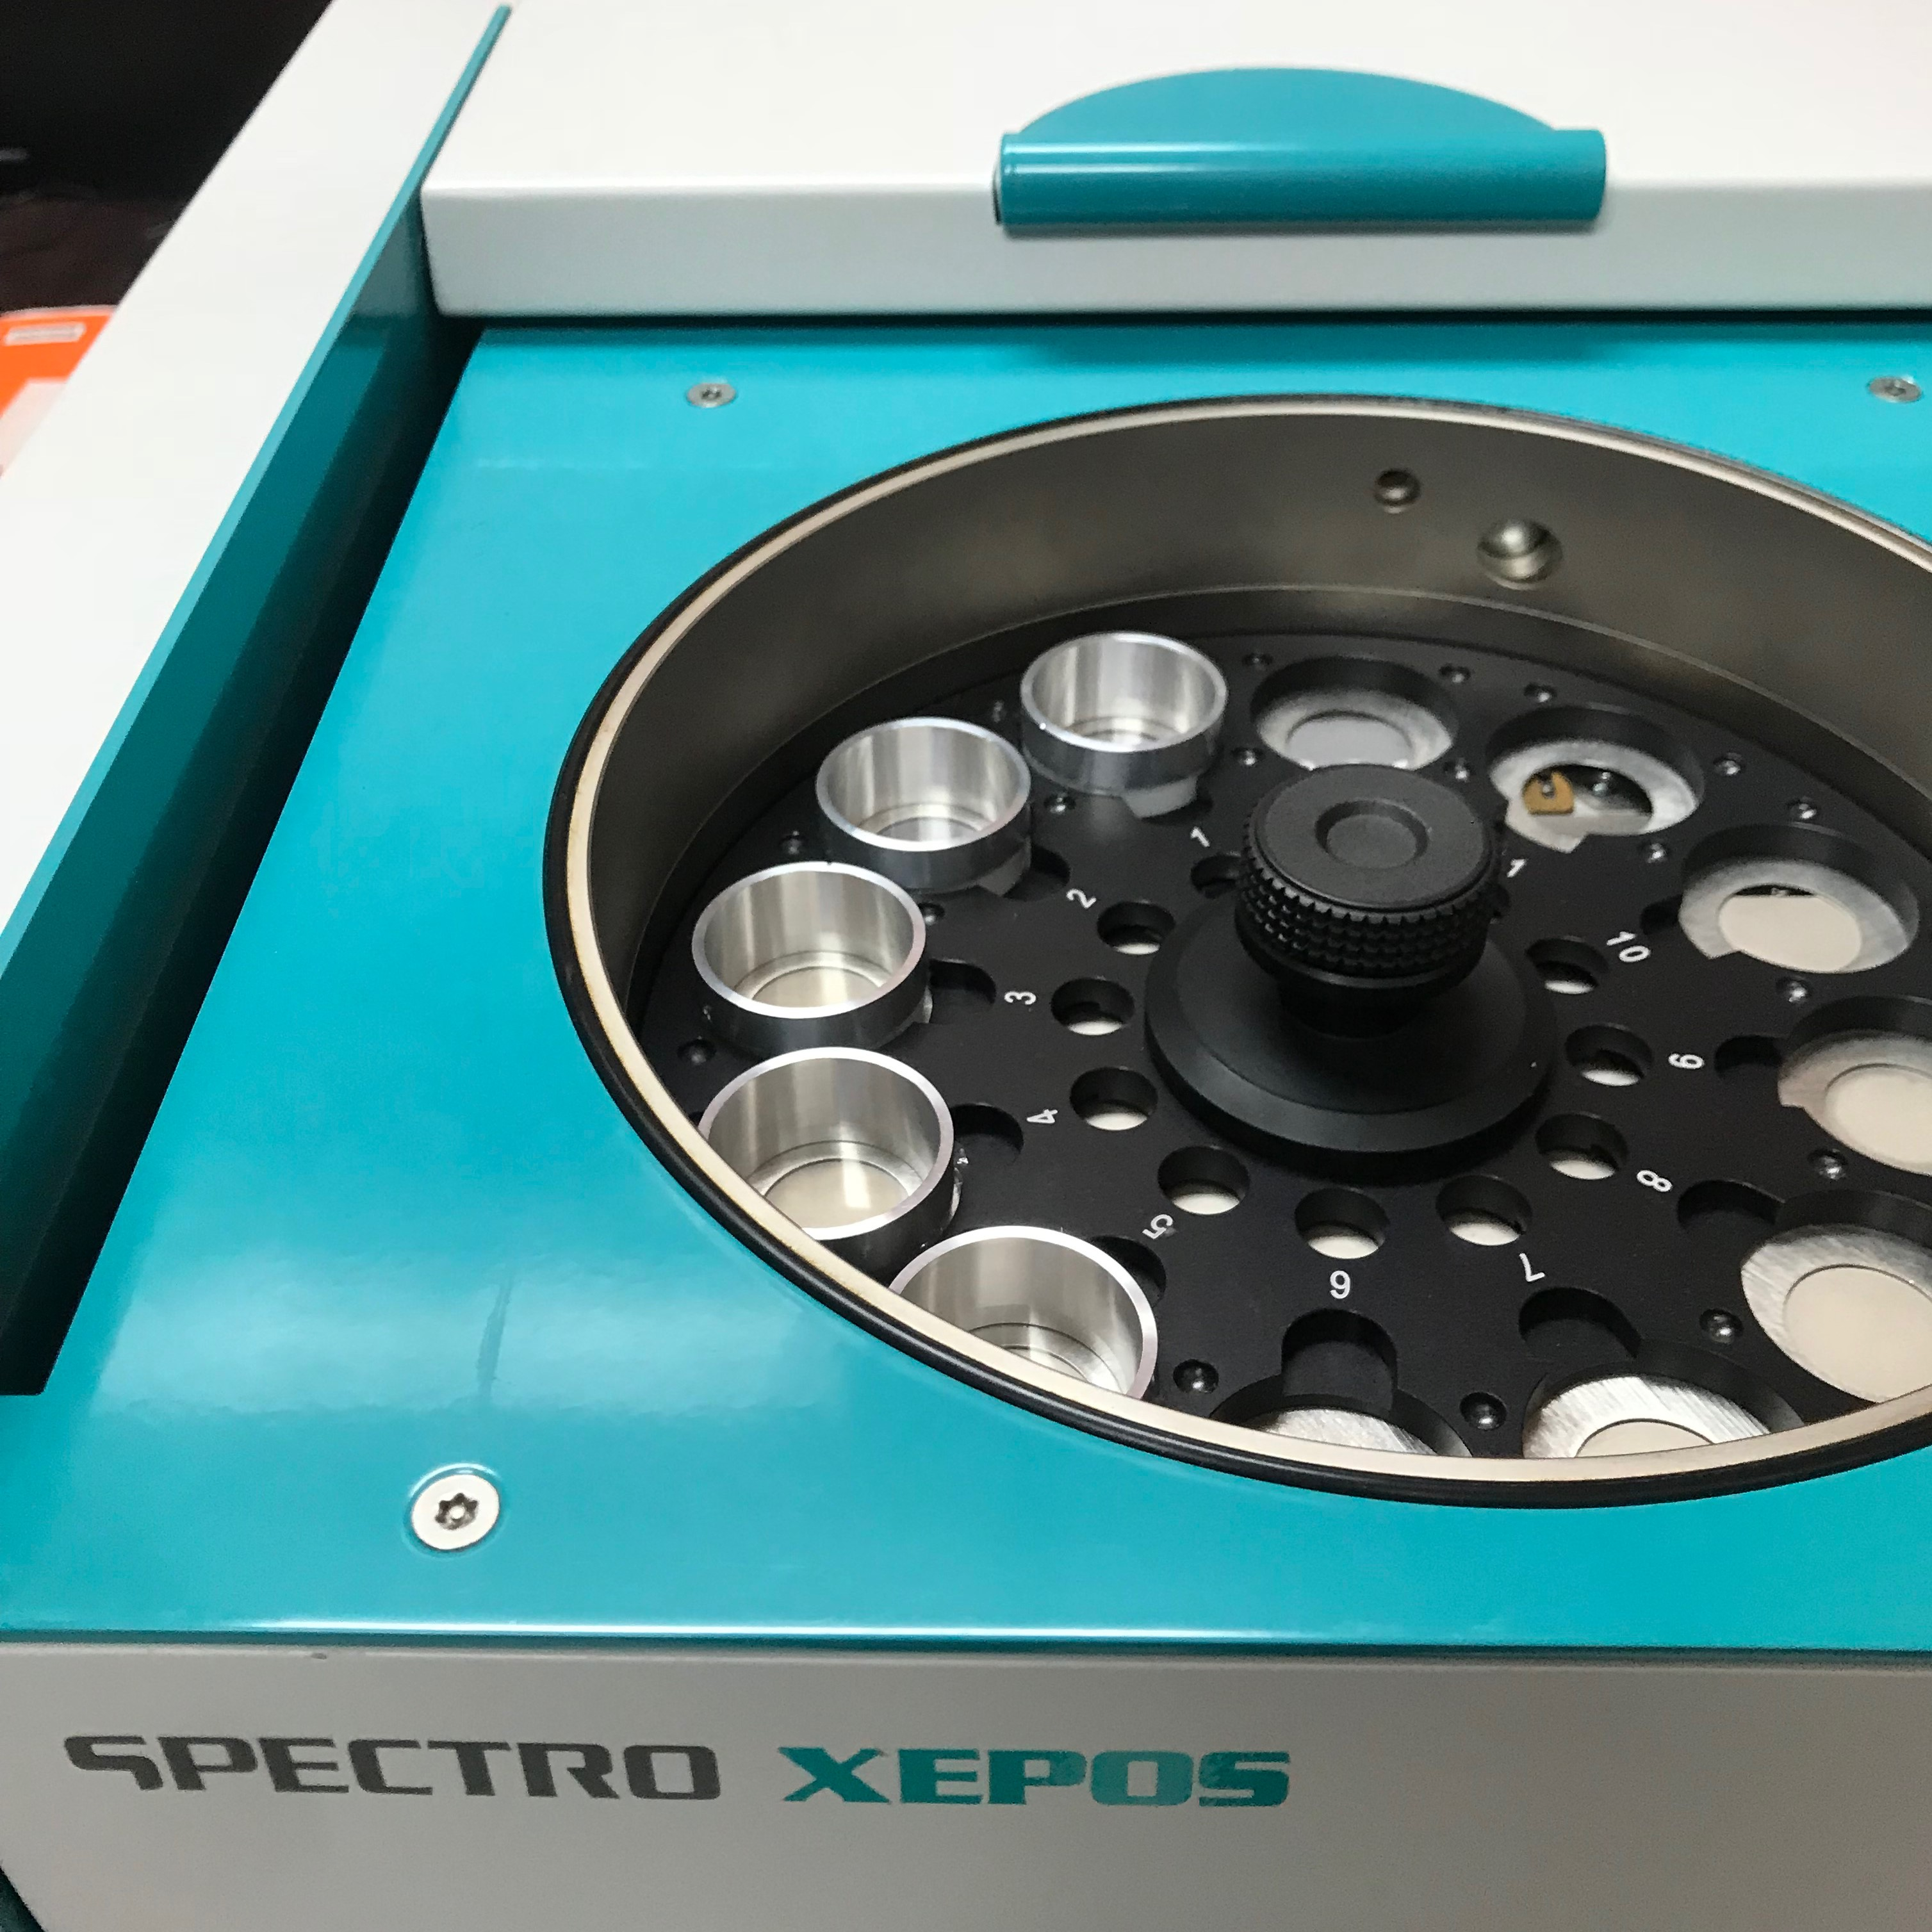
\includegraphics[width=0.35\textwidth]{Imagenes/XEPOS.jpg}
\caption{Vista superior equipo de fluorescencia de rayos X, \textit{SPECTRO XEPOS III}, del LGIG.}\label{Fig-XEPOS}
\end{figure}
	\section{Analizador elemental de carbono y nitrógeno}\label{Secc-CN}
La medida de la concentración de C y N se realizó mediante el analizador elemental por combustión (sección \ref{SubSec-CN-Intro}) \textit{Vario Micro Cube}, marca Elementar (Figura \ref{Fig-Elementar}). La cantidad de masa necesaria por muestra es de $\sim$ 20 mg. El porcentaje de carbono y nitrógeno se calcula a partir de una curva de calibración construida mediante Materiales de Referencia Certificados, y la incertidumbre en la medición se calcula a través de triplicados mediante una ecuación similar a la Ecuación \ref{Eq-SigmaRef}.
\begin{figure}[h]
\centering
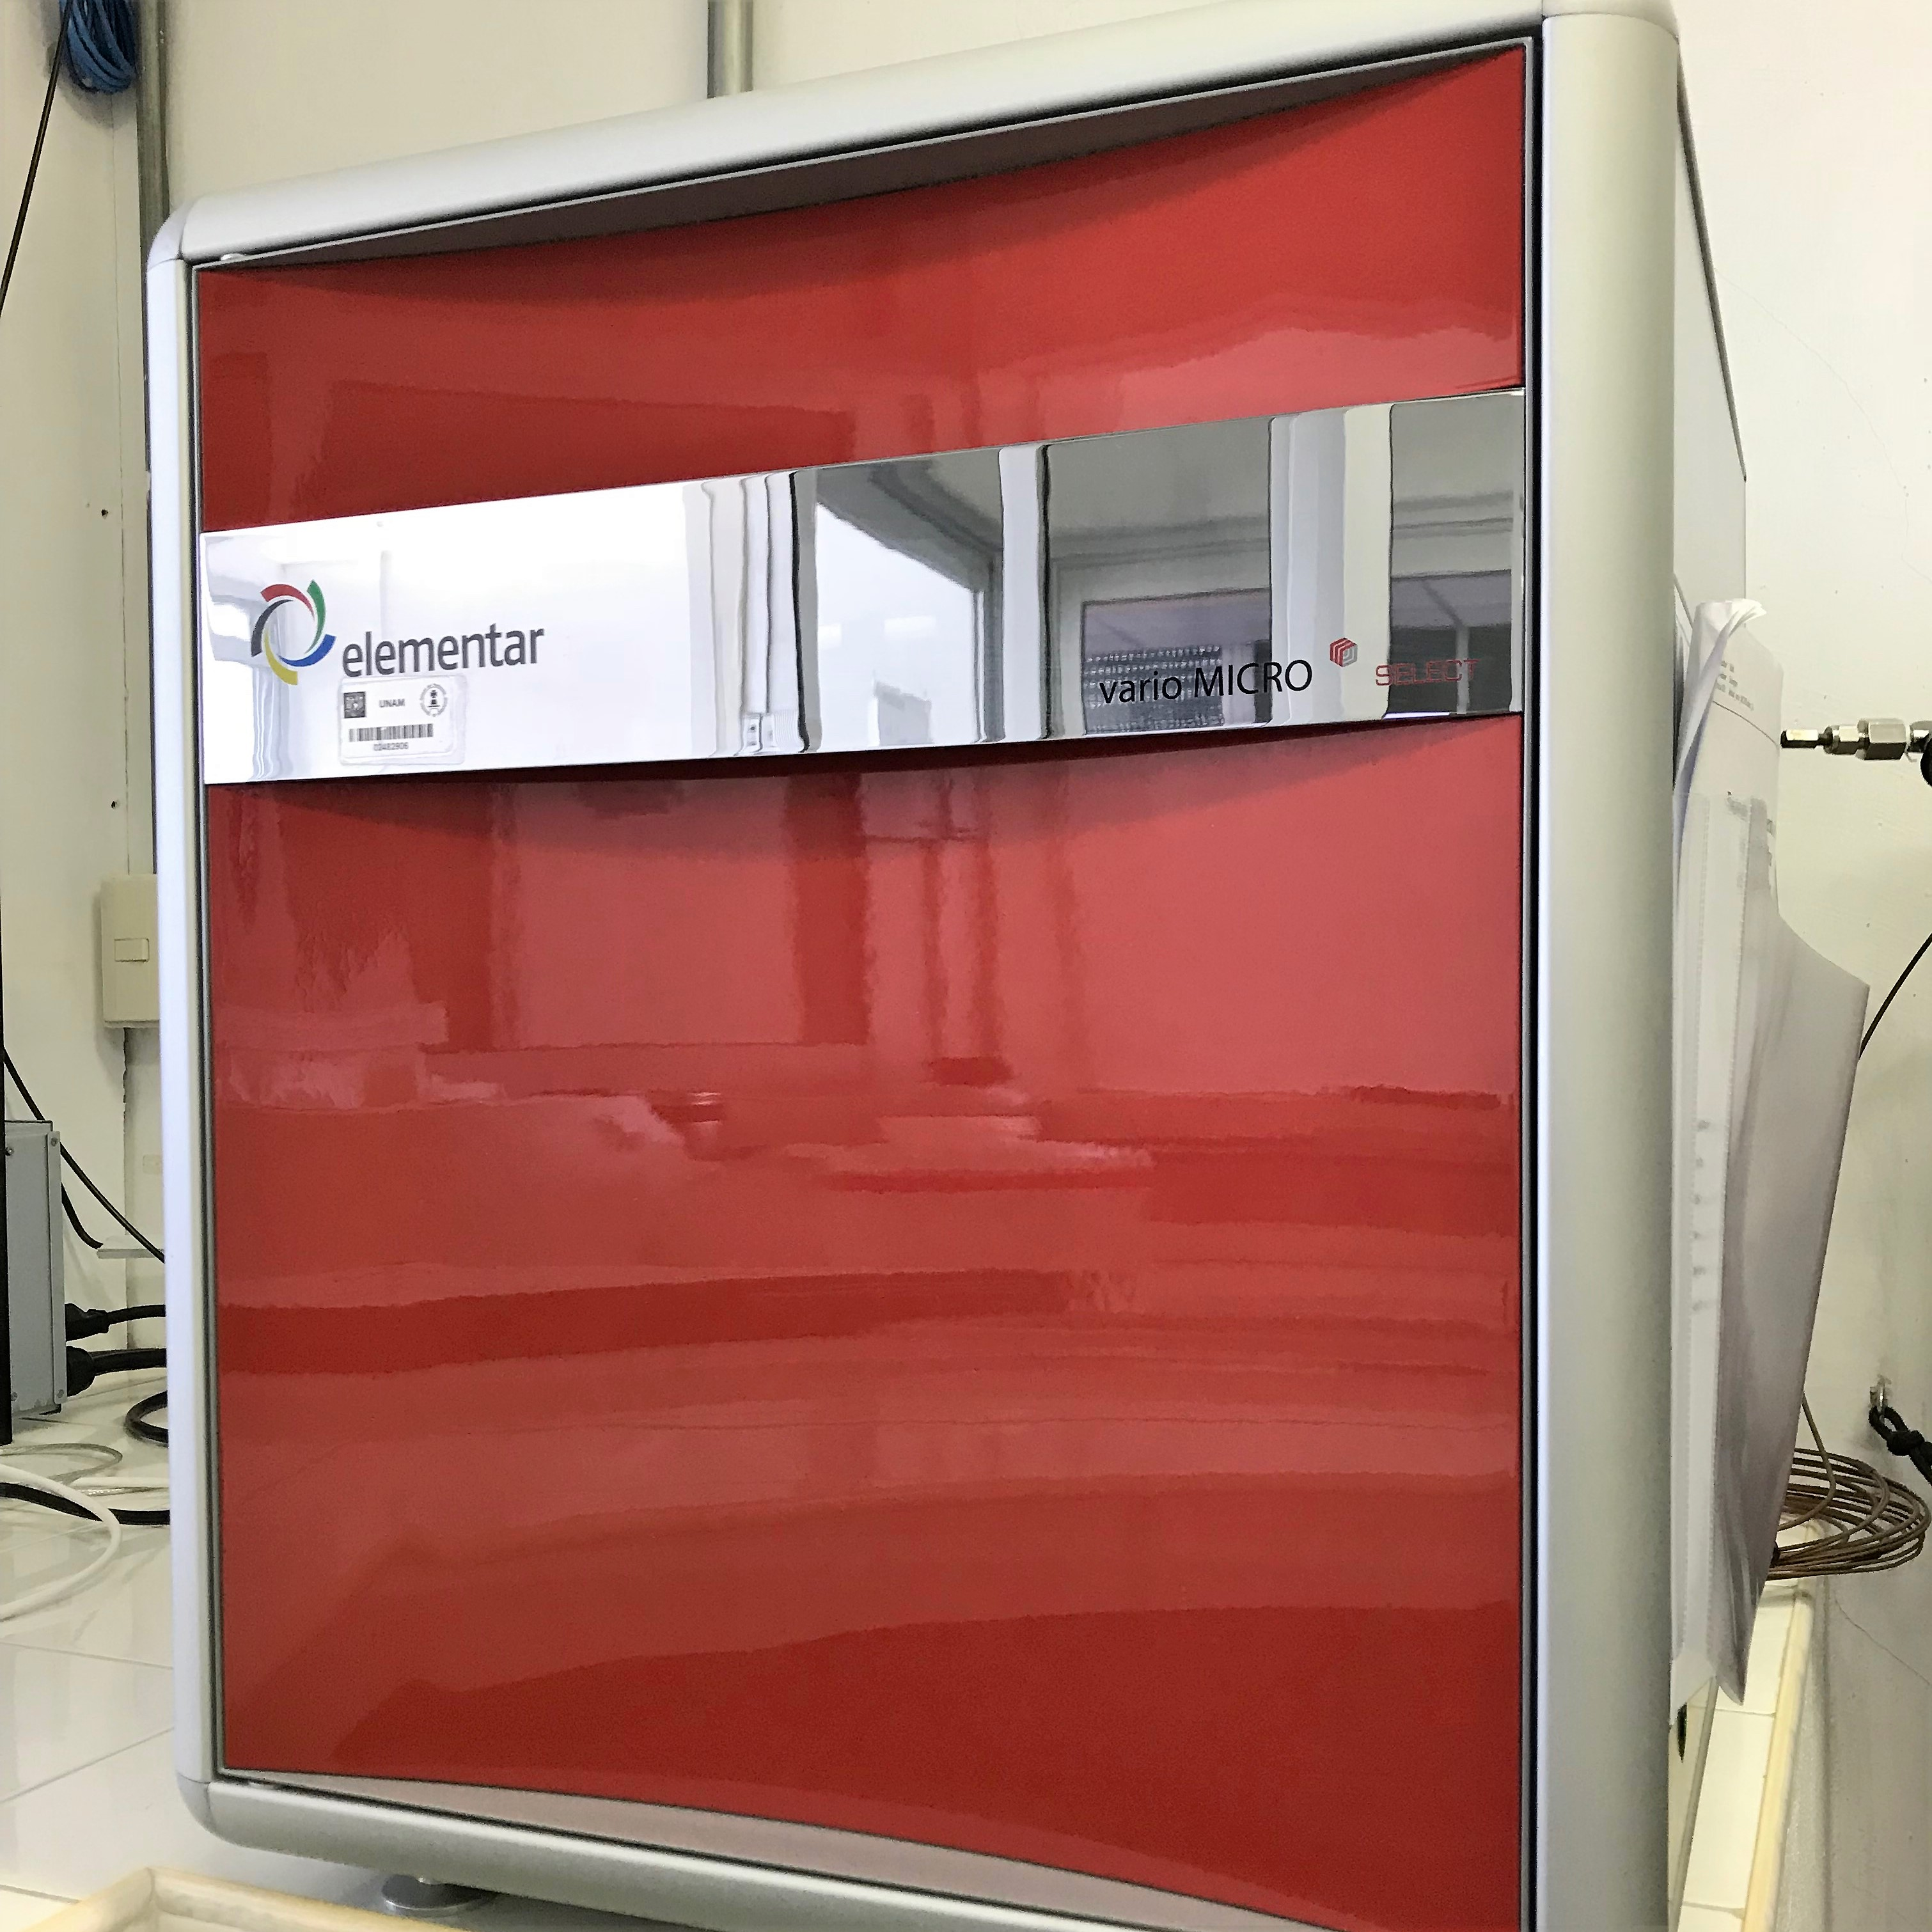
\includegraphics[width=0.35\textwidth]{Imagenes/Elementar.jpg}
\caption{Analizador elemental de carbono y nitrógeno \textit{Vario Micro Cube, Elementar}, empleado en el LGIG.}\label{Fig-Elementar}
\end{figure}
	\section[Definición de la composición elemental]{Definición de la composición elemental}\label{Secc-100Composicion}
Los elementos de la composición de cada sección de un núcleo sedimentario son conocidos excepto para algunos elementos, de los que podemos destacar H y O porque son constituyentes relevantes de la materia orgánica (fundamentalmente C, H y O) y de los carbonatos (Ca, C y O).
\\
\\
El porcentaje de C, N y en especial la relación C/N, se encuentran reportados para  algunos núcleos sedimentarios de zonas costeras, esteros, manglares y lagos, e.g. \cite{ramanathan2010management}, \cite{BARDHAN201590}, \cite{DUNN20082535}, \cite{TUE201887}. Sin embargo, el porcentaje de materia orgánica y su composición presentan una gran variabilidad entre ecosistemas, así como entre las muestras de un mismo núcleos sedimentario, por lo que es necesario determinar estos parámetros para cada muestra.
\\
\\
Para la simulación de la autoabsorción con ANGLE, es necesario conocer el 100 \% de la composición elemental de la muestra. Para ello, se calculó la fracción de composición desconocida y se atribuyó a la misma a la suma de H y O. 
\\
\\
Por ejemplo, si $x_i$ denota la concentración absoluta del elemento $i$, $\bigtriangleup$ denota la incertidumbre asociada y $x_\text{desconocido}$ denota el valor de la composición desconocida, entonces 
\begin{eqnarray}
x_\text{desconocido} &=& 1 - \biggl( x_\text{C} + x_\text{N} +  x_\text{Na} + x_\text{Mg} + \cdots + x_\text{U} \biggr), \\
\bigtriangleup x_\text{desconocido} &=& \sqrt{ 
(\bigtriangleup x_\text{C})^2 +
(\bigtriangleup x_\text{N})^2 +
(\bigtriangleup x_\text{Na})^2 +
(\bigtriangleup x_\text{Mg})^2 +
\cdots +
(\bigtriangleup x_\text{U})^2 }.
\end{eqnarray}
Si se establece que el porcentaje de contribución de oxígeno a la composición desconocida sea del 75 \%, la concentración de O e H y sus incertidumbres son 
\begin{eqnarray}
x_\text{O} = 0.75\times x_\text{desconocido}, & \hspace{1cm} & \bigtriangleup x_\text{O} = 0.75\times \bigtriangleup x_\text{desconocido}, \\
x_\text{H} = 0.25\times x_\text{desconocido}, & \hspace{1cm} & \bigtriangleup x_\text{H} = 0.25\times \bigtriangleup x_\text{desconocido}.
\end{eqnarray}
Así, existen dos composiciones: 
\begin{itemize}
\item composición de referencia (agua) y 
\item composición corregida establecida mediante el procedimento descrito anteriormente. 
\end{itemize}
Las cantidades que se relacionan con las composiciones son la eficiencia $\epsilon$, la actividad específica $A$ de un radionúclido y los resultados del fechado. La actividad corregida $A_\text{corr}$ se relaciona con la eficiencia corregida $\epsilon_{\text{corr}}$, la eficiencia de referencia $\epsilon_\text{ref}$ y la actividad de referencia $A_\text{ref}$ mediante
\begin{equation}\label{Eq-ActividadCorregida}
A_\text{corr} = \dfrac{\epsilon_\text{ref}}{\epsilon_{\text{corr}}}\,A_\text{ref}.
\end{equation}
	\section{Zonas de estudio}\label{Secc-ZonasSeleccionadas}
Las composiciones elementales de cada núcleo sedimentario dependen de un gran número de variables, tales como el tipo de ecosistema, el entorno geológico, la distancia a la costa, entre otros. Para el presente trabajo se seleccionaron núcleos sedimentarios pertenecientes a ecosistemas contrastantes (lagos, manglares, zona costera y mar abierto) de zonas diversas de México (ambiente terrígeno, Océano Pacífico, Golfo de México y Mar Caribe). Estos se encuentran consignados en la Tabla \ref{Table-ZonasSeleccionadas} y Figura \ref{Fig-Mapa}. 
\begin{table}[h]
\centering
\caption{Información de los núcleos sedimentarios analizados, incluyendo código, nombre extenso, zona geográfica de recolección y Gran Ecosistema Marino (LME) al que pertenece.}\label{Table-ZonasSeleccionadas}
\begin{tabular}{|c|c|c|c|}
	\hline								
\rowcolor{Blue2}	Código 	&	Nombre extenso	&	Zona geográfica	& 	LME	 \\	\hline
\rowcolor{Blue1}	GOMRI-500	&	Golfo de Mexico 500	&	Golfo de México	&	5	 \\	
\rowcolor{Blue1}	EU-VIII	&	Estero de Urias VIII	&	Sinaloa, Mazatlán	&	4	 \\	
\rowcolor{Blue1}	PCm	&	Punta Caracol manglar	&	Punta Caracol, Quintana Roo	&	12	 \\	
\rowcolor{Blue1}	LTAF	&	Laguna de Términos, Atasta Franja	&	El Carmén, Campeche	&	5	 \\	
\rowcolor{Blue1}	SAMO-14-2	&	Santa María del Oro 14-2	&	Santa María del Oro, Nayarit	&	NA 	 \\	
\rowcolor{Blue1}	TEHUA-XII	&	Tehuantepec  XII	&	Golfo de Tehuantepec	&	11	 \\	\hline
\end{tabular}
\end{table}
\begin{figure}[h]
\centering
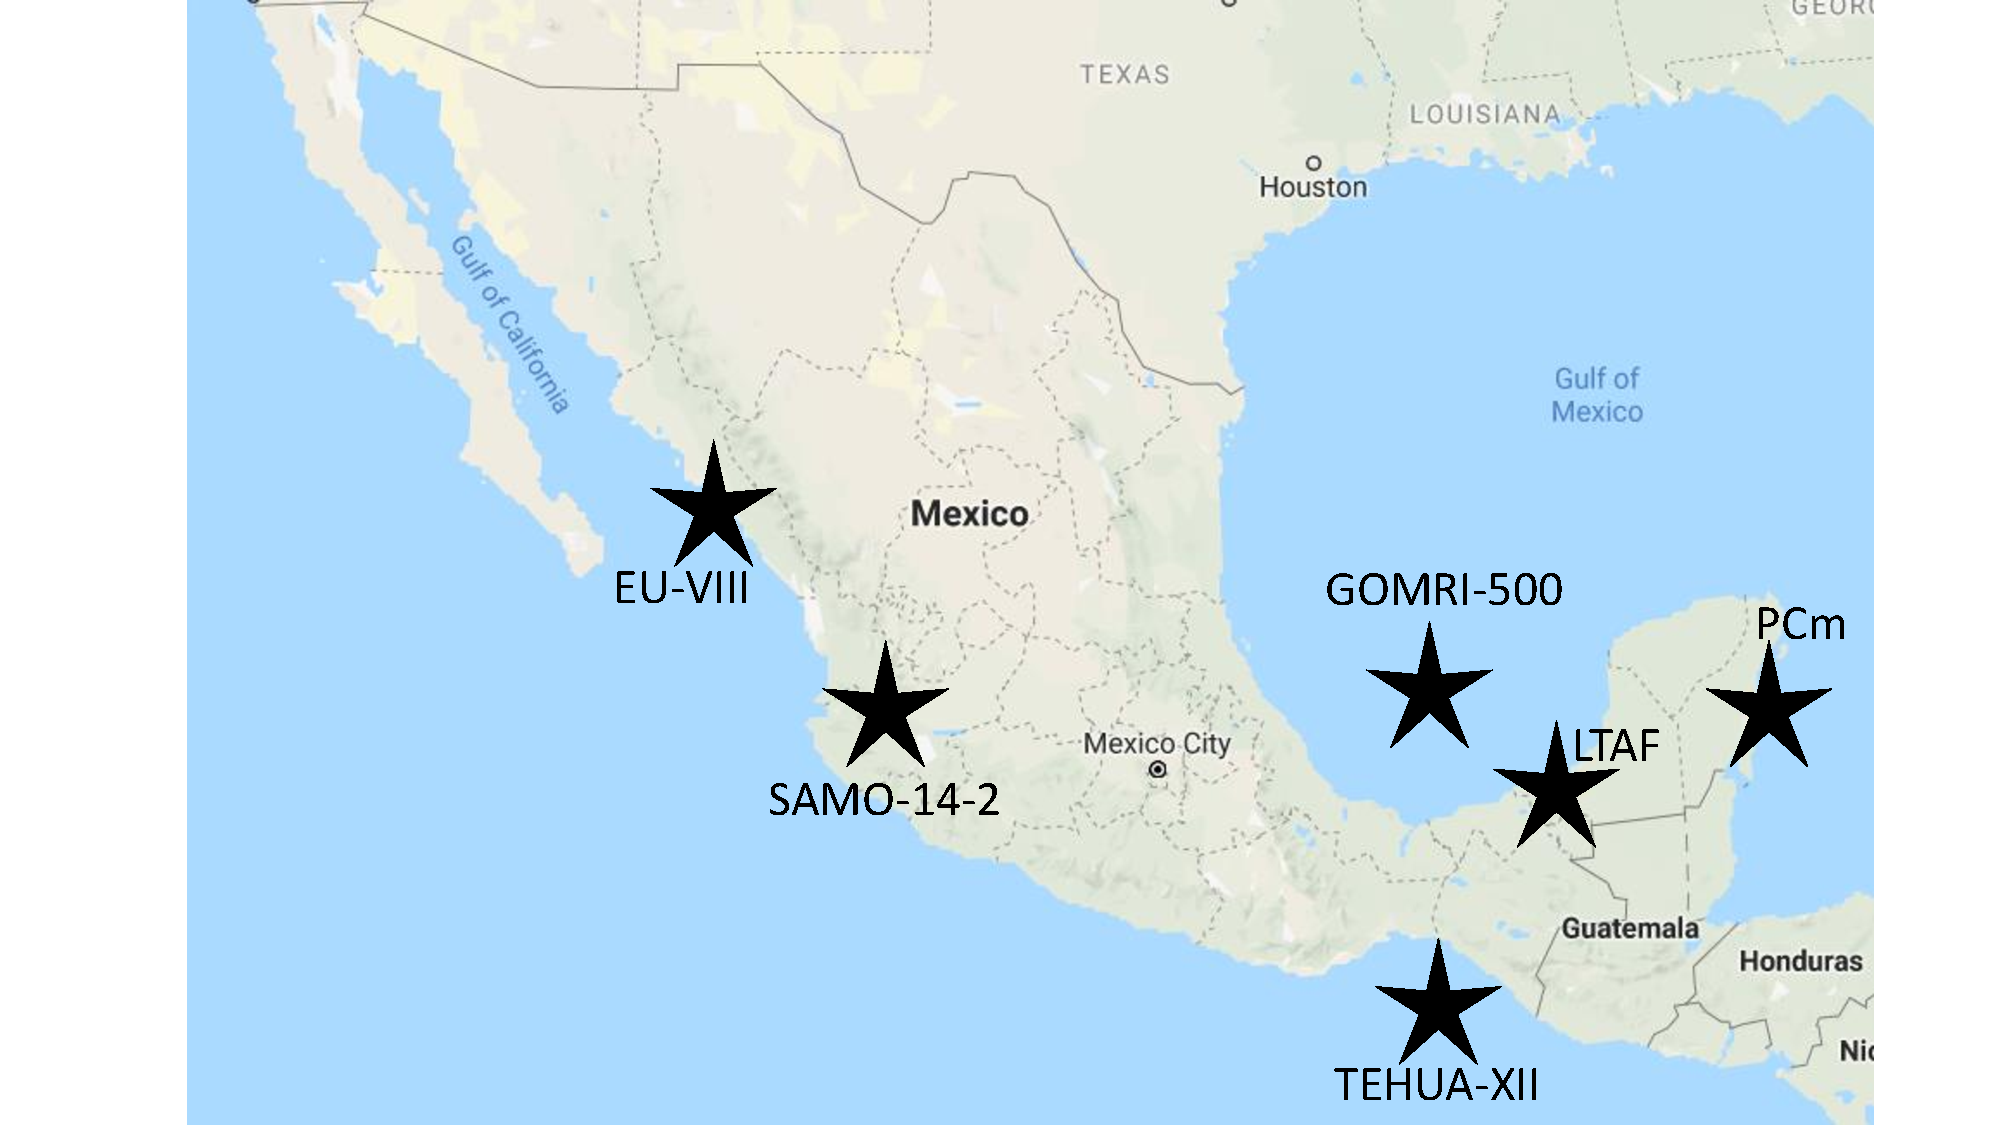
\includegraphics[width=\textwidth]{Imagenes/Mapa_Nucleos_Seleccionados.pdf}
\caption{Ubicación geográfica de los núcleos sedimentarios seleccionados para el presente trabajo.}\label{Fig-Mapa}
\end{figure}
\section[Códigos desarrollados]{Códigos desarrollados}\label{Secc-Codigos}
\subsection{Tratamiento de datos}
Los datos experimentales medidos de una sección de un núcleo sedimentario incluyen la actividad de los radionúclidos \PbCero\, y \PbCuatro\, obtenidos mediante espectrometría de rayos gamma y la composición elemental (Sección \ref{Secc-EspectrometriaGamma}) determinada por espectrometría de fluorescencia de rayos X (Sección \ref{Secc-EspectrometriaXRF}) y análisis elemental C-N (Sección \ref{Secc-CN}). Se generó un código en el lenguaje de programación R para leer, limpiar e integrar la información disponible para cada núcleo sedimentario, incluyendo la estimación del 100 \% de la composición elemental de cada sección (Sección \ref{Secc-100Composicion}) y el cálculo de la eficiencia corregida $\epsilon_\text{corr}$ para el sistema detector - muestra.
\\
\\
El código contempla los siguientes pasos: 1) limpiar los archivos originales, 2) definir 100 \% de la composición, 3) generar un archivo con la información relacionada con el tipo de detector, contenedor, composición, energías de interés, parámetros de ANGLE, 4) ejecutar ANGLE, y 5) leer los resultados de ANGLE.
\subsubsection{Manipulación de archivos originales}
La limpieza de los archivos generados por cualquier equipo se debe realizar debido a la posibilidad de resultados repetidos, errores de captura, entre otras. Esto debe ser realizado de forma automática para minimizar la manipulación manual de los resultados. En este trabajo se utilizaron resultados del analizador elemental C-N, XRF y espectrometría de rayos gamma.
\\
\\
La manipulación del archivo original de C-N se centra en la identificación de las filas a analizar y en el cálculo de las incertidumbres a través de los triplicados realizados. La identificación de las filas a analizar es necesario porque en un mismo archivo se almacenan los resultados de muestras de diversos núcleos. 
\\
\\
Para los resultados XRF, el código se enfoca en identificar las filas a analizar, eliminar valores negativos o valores reportados como menor o igual que el límite de detección, y convertir las concentraciones reportadas en porcentaje o partes por millón a concentraciones absolutas. Por ejemplo, una concentración de 5 \% de sodio significa una concentración absoluta de 0,05 de sodio. 
\\
\\
Los resultados de la espectrometría de rayos gamma son complejos pues albergan una gran cantidad de información. La finalidad del código es extraer información de cada archivo, correspondiente a una sección medida. La información extraída es la actividad, su incertidumbre y el límite de detección de los radionúclidos de interés, la fecha de medida, el detector y la geometría utilizada, el archivo de calibración, el método de análisis, el archivo de fondo utilizado, la masa y la densidad. 
\subsubsection{Definición de la composición de cada sección}
El procedimiento se describe en la Sección \ref{Secc-100Composicion}.
\subsubsection{Generación de archivo para ejecutar ANGLE}
La ejecución de ANGLE implica generar un archivo.SAVX que contiene toda la información requerida para su ejecución: detector (G1, G2, G3 o G4), vial (2 mL o 4 mL),  material (composición corregida) y curva de referencia.  Además, es necesario generar un archivo de bash (.sh) que contiene la instrucción de ejecutar ANGLE desde R. 
\subsubsection{Lectura de los resultados de ANGLE}
ANGLE genera archivos (.OUTX) que contienen el ángulo sólido efectivo y la eficiencia para las energías seleccionadas (Sección \ref{SubSec-ANGLE}). Esta eficiencia corregida $\epsilon_\text{corr}$, que tiene en cuenta el 100 \% de la composición y la densidad de la muestra, junto con la eficiencia de referencia $\epsilon_\text{ref}$ y la actividad de referencia extraída de los archivos .rpt $A_\text{ref}$, permite corregir la actividad $A_\text{corr}$ mediante la Ecuación \ref{Eq-ActividadCorregida}.
\subsection[Incertidumbre de eficiencia corregida ]{Incertidumbre de la eficiencia corregida}\label{SubSec-IncertidumbreEffMonteCarlo}
Se estimó que la mayor fuente de incertidumbre en la eficiencia corregida es la incertidumbre de la composición de la muestra (ver Apéndice \ref{SecResulIncertidumbreEffMonteCarlo}). Para calcularla, se realizó una simulación Monte Carlo variando la composición de cada elemento según una distribución normal, a partir de la concentración medida y su incertidumbre. Se hizo el mismo ejercicio con la densidad de la muestra. Esta simulación se realizó con una composición corregida de 50 \% oxígeno - 50 \% hidrógeno para una sección escogida al azar. La incertidumbre de la eficiencia corregida se calculó como la desviación estándar de los resultados generados mediante la simulación para cada una de las composiciones. 
